\section{Эксперементальный раздел}
В данном разделе произведен ряд эксперементов с полученным, в ходе написания проекта, программным обеспечением.
Для проведения серии эксперементов необходимо подготовить набор тестовых входных данных, представляющих собой тридцать электронных документов на русском языке, формата PDF.
Все работы учавствующие в экперементе взята с сайта 
Для тестов отбираются тексты с указанными ключечевыми словами с целью сопоставления авториских КС с полученными из метода.

Для обеспечения качества проводимых эксперементов необходима указать критерии по которыму будет проиводиться отбор документов:
\begin{enumerate}
	\item документ должен содержать в себе текст, а не отсканированные изображения страниц ранее опубликованных работ, по скольку это приводит к невозможности прочтения документа;
	\item информация содержащаяся в документе должна быть целой, то есть принадлежать одной работе.
\end{enumerate}

\subsection{Исследование зависимости результата от параметра n}
Целью данного исследования является изучение зависимости результата извлечения ключевых слов, от параметра n, отвечающего за размер используюемых n-грамм.
На рисунке \ref{fig:experiment24} представлены результаты работы алгоритма при n варьирующемся от 1 до 3.

\begin{figure}[!h]
	\centering
	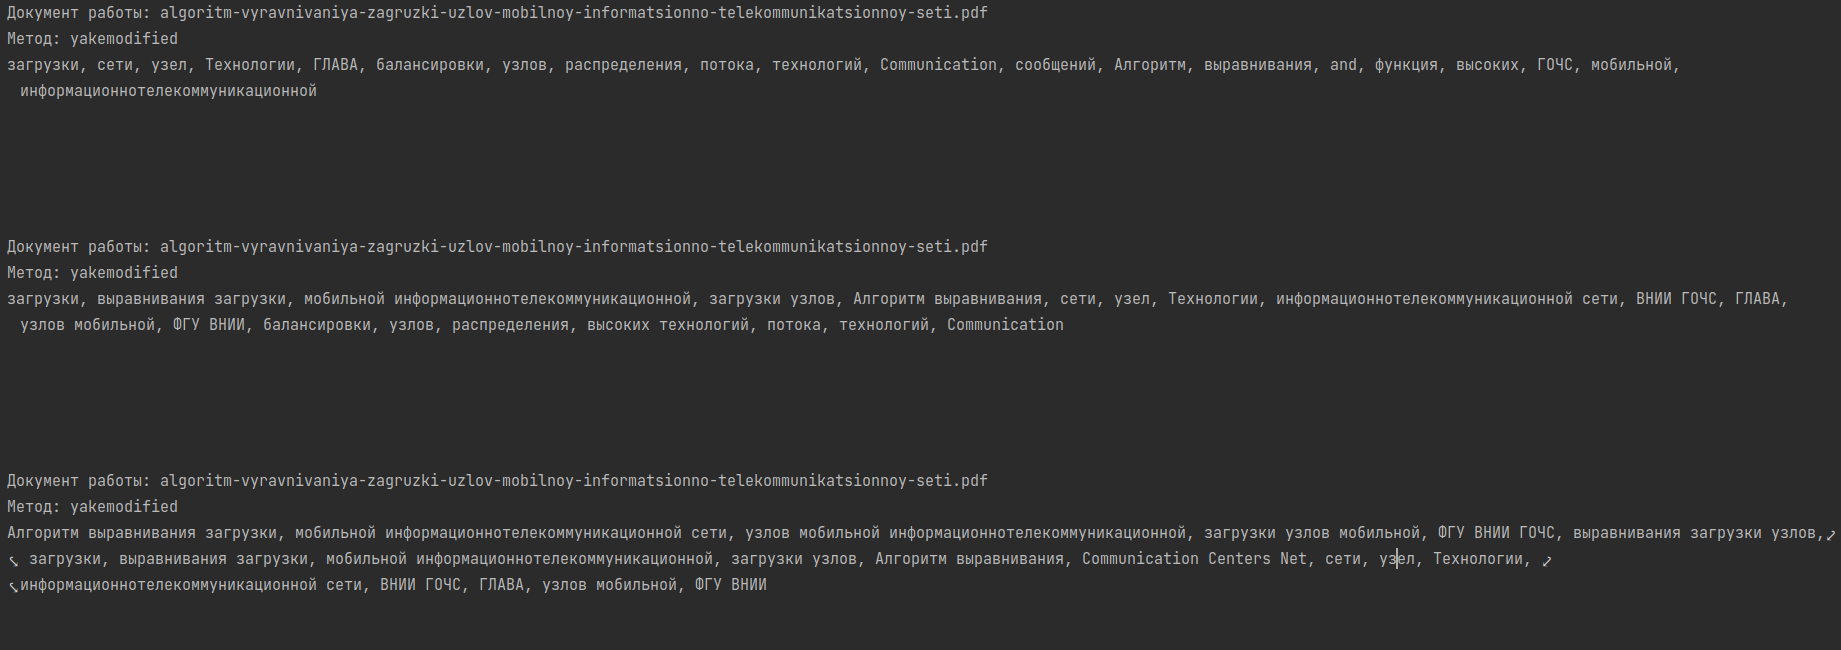
\includegraphics[width=1\linewidth]{src/img/experiment/experiment_2_4}
	\caption{Результат работы алгоритма от параметра n}
	\label{fig:experiment24}
\end{figure}
Как и предпологалось в зависимости от параметра n будут появляться многокомпонентные термины, размер которых зависит от данного параметра.
При n = 1, однокомпонентные КС, при n = 2 двухкомпонентные, при n = 3 трехкомпонентные.
Примером расширения ключевого слова является "информационнотелекоммуникационной" который преобразуется в "информационнотелекоммуникационной сети" и "мобильной информационнотелекоммуникационной" (рисунок \ref{fig:experiment24}), а затем в "мобильной информационнотелекоммуникационной сети"

\subsection{Исследование точности метода}
В рамках данного эксперемента оценивается результат работы модифицированного метода Yakе на ранее подготовленных тестовых данных, путем оценки процентного пересечения ключевых слов отмеченными авторами текста с КС полученными в итоге отработки метода.

Для алгоритма Yake были выставлены параметры отображенные на рисунке \ref{fig:experiment11}
\begin{figure}[!h]
	\centering
	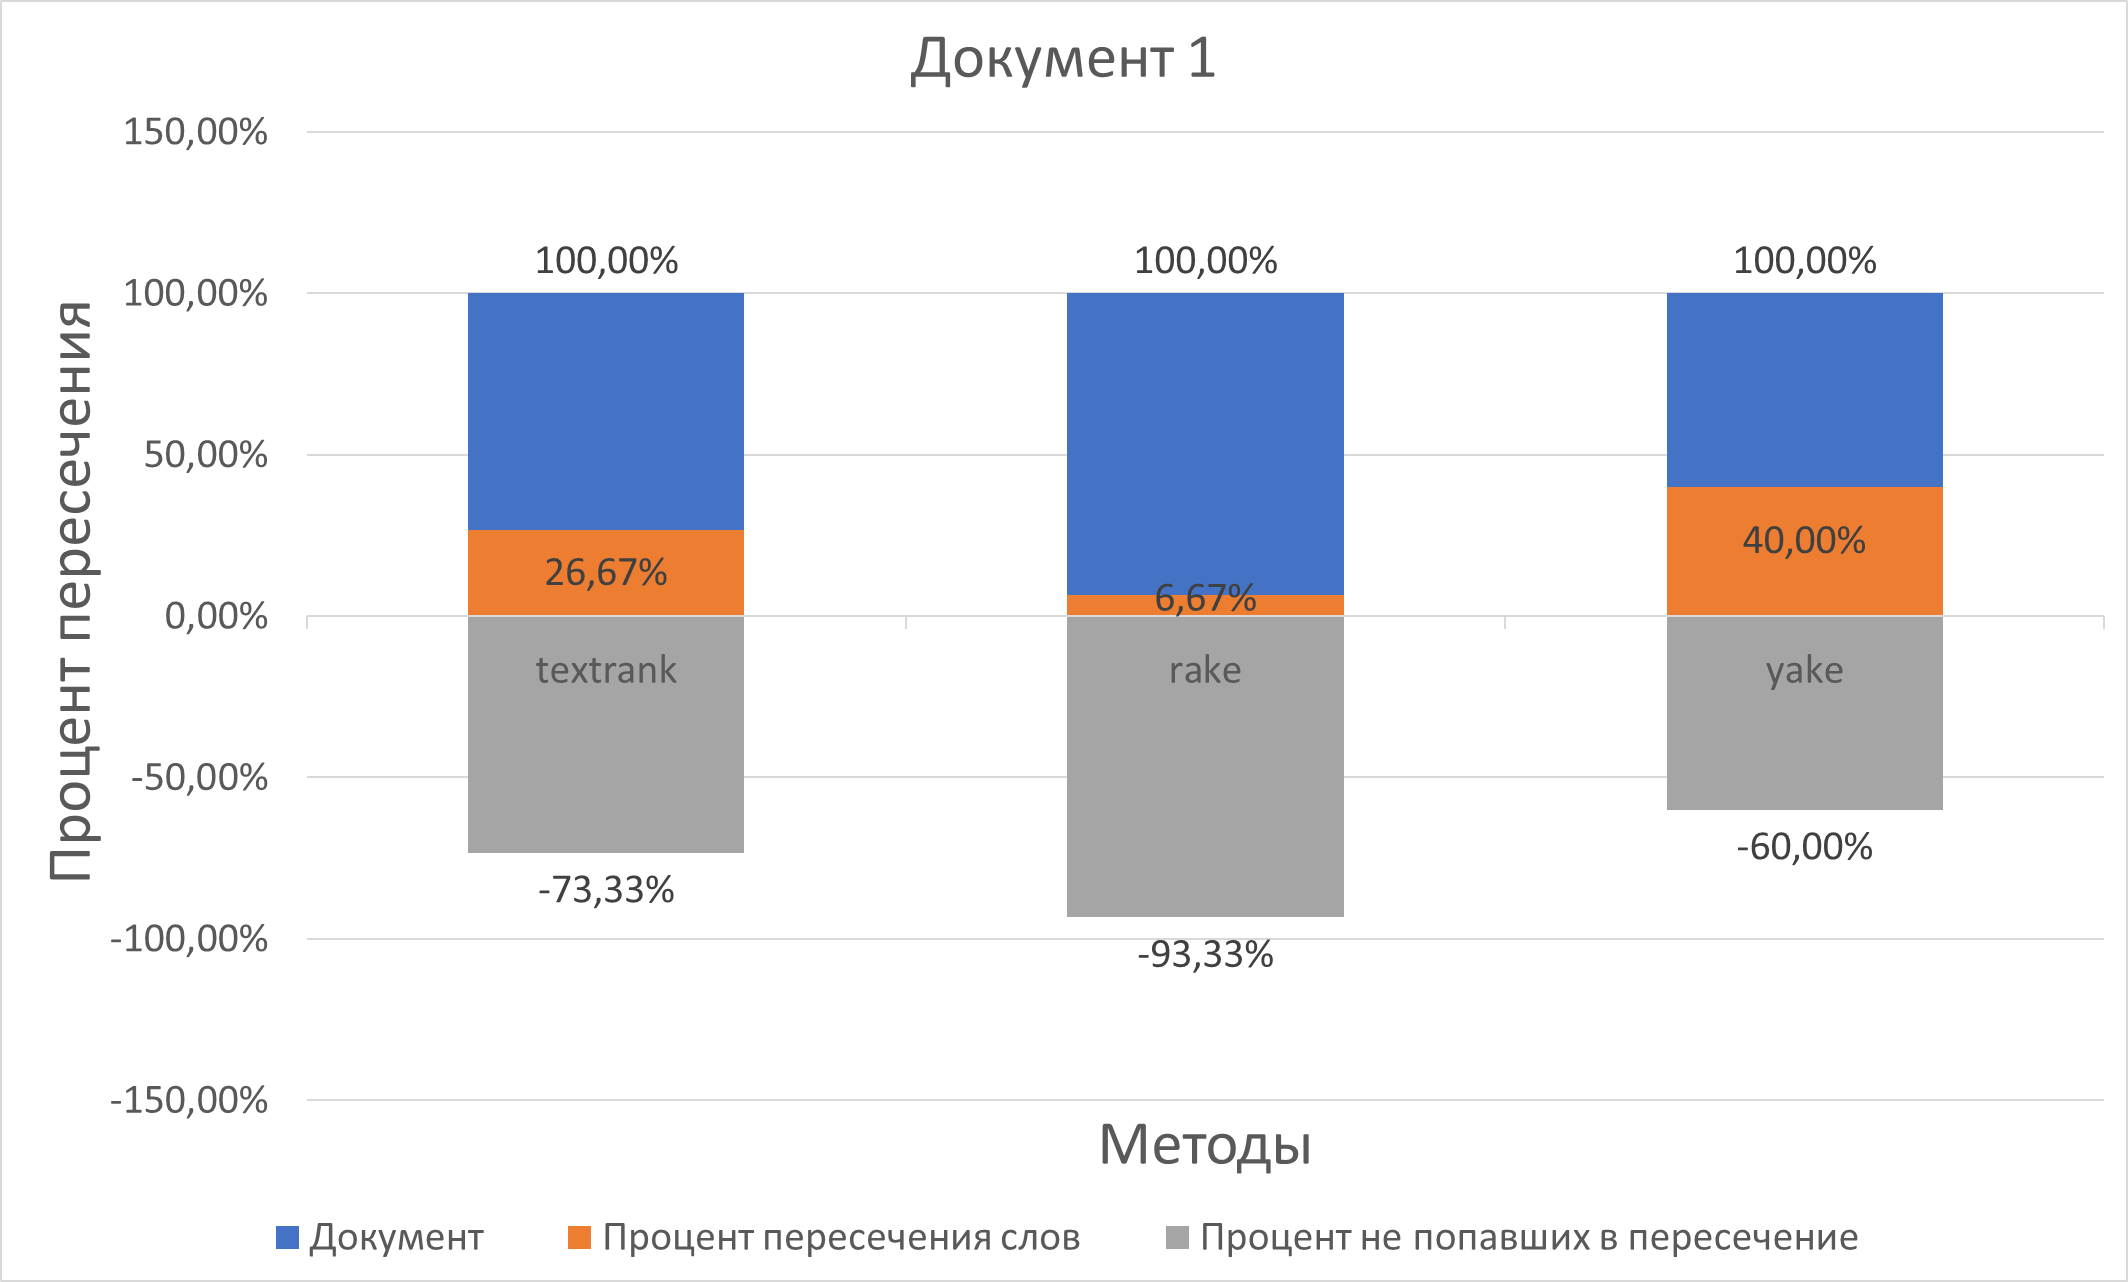
\includegraphics[width=1\linewidth]{src/img/experiment/experiment_1_1}
	\caption{Параметры модифицированного метода Yake}
	\label{fig:experiment11}
\end{figure}

На рисунке \ref{fig:experiment12} представлен результат сравнения ключевых слов предоставленных авторами документов с КС полученные путем извлечения.
В ходе данного эксперемента было установлено что процент пересечения оригинальных слов и полученных путем извлечения составляет $33\%$.
\begin{figure}[!h]
	\centering
	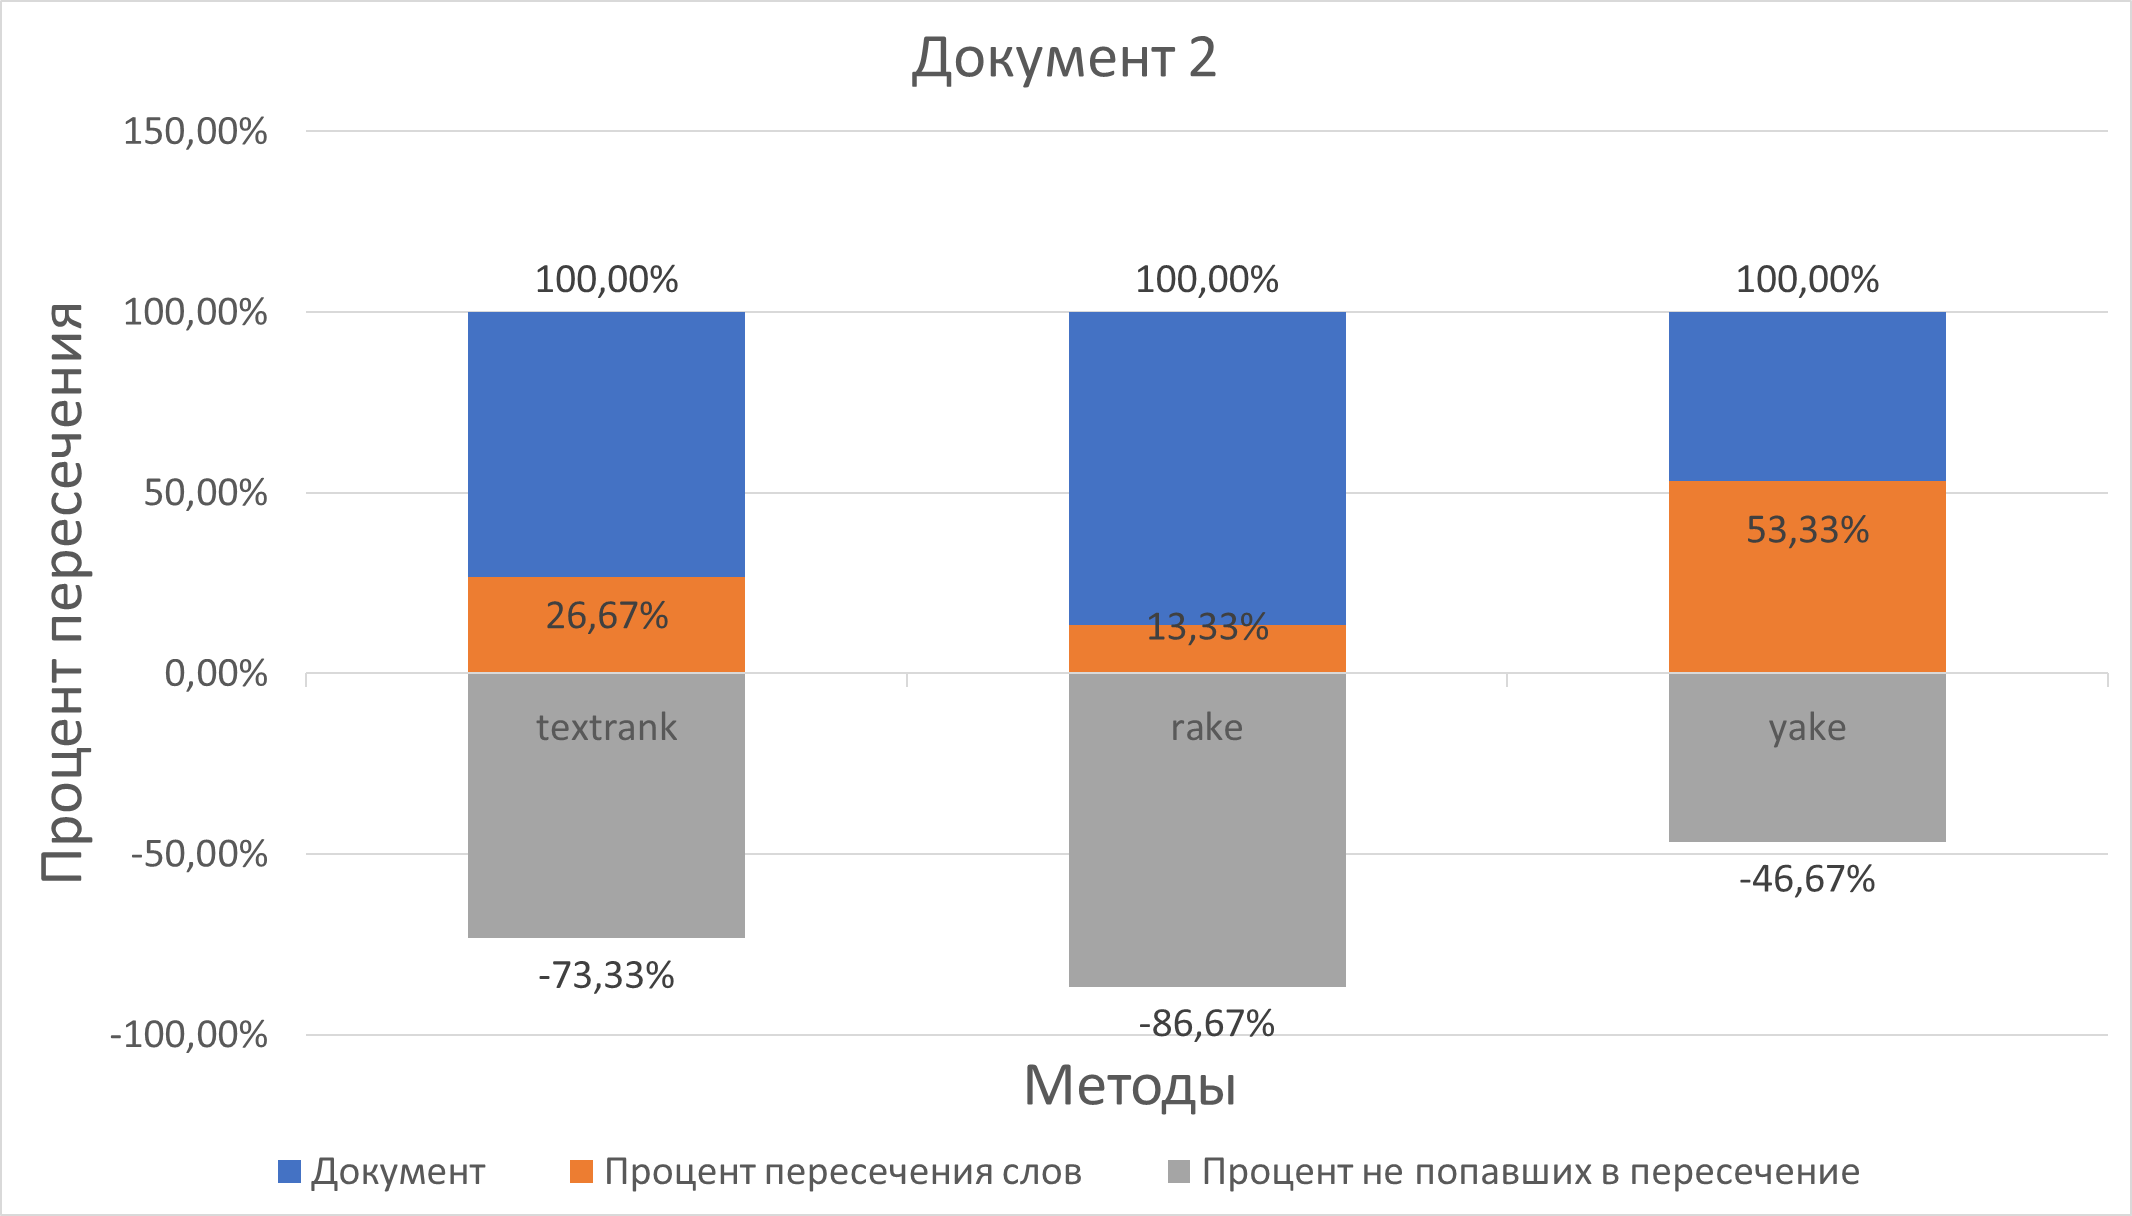
\includegraphics[width=1\linewidth]{src/img/experiment/experiment_1_2}
	\caption{Результат пересения ключевых слов}
	\label{fig:experiment12}
\end{figure}

\subsection{Исследование эффективности метода}
Для изучения эффективности метода, полученного в рамках данной работы, были выбраные еще несколько алгоритмов:
\begin{enumerate}
	\item Rake;
	\item Bert;
\end{enumerate}
Метрикой эффективности будет являться процент пересечения ключевых слов, полученных в результате работы выше перечисленных методов, с КС, указанных авторами текстов.



\subsection{Вывод}
В результате проведения исследовательской работы над разработанным решением было установлено, что все требования, поставленные к алгоритму, соблюдены.
Алгоритм способен на извлечение многокомпонентных ключевых слов из документов на русском языке.
